\chapter{\textsc{SETL2}}
The concepts from set theory introduced in the last chapter are quite abstract and
therefore are difficult to grasp at the beginning.  In order to facilitate the
assimilation of these concepts we introduce the programming language \textsc{Setl}.  The
name is short for \underline{set} \underline{l}anguage. As \textsc{Setl} is based on set
theory, working with \textsc{Setl} increases the understanding of set theoretical
concepts.  Furthermore, programming in \textsc{Setl} is quite rewarding, as many problems,
whose solution would take long and complicated programs  in programming languages like \texttt{C} or
\textsl{Java},  have short and elegant solutions when programmed in \textsc{Setl}.

Due to time constraints, I won't be able to discuss every feature of \textsc{Setl}.
The reader interested in the features not covered in this lesson is referred to the
literature for further information.  
The article \cite{dewar79} provides an introduction, while \cite{snyder90b} covers the
complete language.  You can find these articles on the following web page:
\\[0.2cm]
\hspace*{1.3cm}
\texttt{http://wwwlehre.dhbw-stuttgart.de/\symbol{126}stroetma/setl2.html}
\\[0.2cm]
This web page also provides a guide to install  \textsc{Setl2}, which is the variant of
\textsc{Setl2} that we will use in this lecture.

\section{Introduction to \textsc{Setl2}}
This section demonstrates the basic features of \textsc{Setl} using simple examples.
We start with the program \texttt{hello.stl} shown in figure
\ref{fig:hello} on page  \pageref{fig:hello}.  The line numbers in this figure are not
part of the program.  I have included them in order to be able to refer to individual lines.
The program \texttt{hello.stl} in figure \ref{fig:hello} prints a greeting message onto the screen.

\begin{figure}[!ht]
  \centering
\begin{Verbatim}[ frame         = lines, 
                  framesep      = 0.3cm, 
                  labelposition = bottomline,
                  numbers       = left,
                  numbersep     = -0.2cm,
                  commandchars  = \\\{\},
                  xleftmargin   = 0.8cm,
                  xrightmargin  = 0.8cm
                ]
    -- \emph{My first \textsc{Setl} program.}
    program main;
        print("Hello world!");
    end main;
\end{Verbatim}
\vspace*{-0.3cm}
  \caption{A simple \textsc{Setl} program.}
  \label{fig:hello}
\end{figure} 

If the program from figure \ref{fig:hello} is stored in a file with the name
\texttt{hello.stl}, then in order to compile and execute this program, we need
to execute the following commands.
\begin{enumerate}
\item \texttt{stll -c setl2.lib}

      This commands creates  a library in the current directory.  In the beginning, this
      library is empty. 
      The programs  that we are going to develop will later be added to this library.
      As long as all our program files are put in the same directory, we get by with just one
      library.  Therefore, this command has to be executed only once. 
\item \texttt{stlc hello.stl}

      This command compiles the \textsc{Setl} program from the file 
      ``\texttt{hello.stl}'' and adds the compiled version of it to the library created in
      the first step.
\item \texttt{stlx main}

      This command executes the program with the name ``\texttt{main}'' from the library.
      As a result, the program should print the following message:
      \\[0.2cm]
      \hspace*{1.3cm}
      \hspace*{1.3cm} \texttt{Hello world!}
\end{enumerate}
Let us discuss the details of the program shown in figure
\ref{fig:hello} on page \pageref{fig:hello}.
\begin{enumerate}
\item The first line is a comment.  In \textsl{Setl}, comments are started with the
      the  double dash  ``\texttt{--}''.  Everything between ``\texttt{--}'' and the end of
      the line is considered a comment and ignored by the compiler.
\item The second line is the  \emph{program declaration}.  This declaration defines the
      \emph{name} of the program.  In \textsc{Setl} all programs are stored in one
      library.  Therefore, we have to assign  a name to every program in order to be able
      to look up the program in the library later.

      The  program declaration starts with the keyword ``\texttt{program}'', followed
      by the name of the  program.  In general, a program name can be any string consisting of
      letters, digits and the underscore character ``\texttt{\_}'' that begins with a
      letter.  However, we will be lazy and just call all our programs ``\texttt{main}''.
      Note that \textsc{Setl} is not case sensitive:  Therefore, the names ``\texttt{main}'',
      ``\texttt{Main}'', or even ``\texttt{MAIN}'' all refer to the same name.   This is
      also true for variable names:  Both ``\texttt{x}'' and ``\texttt{X}'' denote the
      same variable!  However, the programs presented in this lecture will never make use
      of case insensitivity.

      The declaration in the second line is terminated with a semicolon ``\texttt{;}''.  
      In \textsc{Setl}, all declarations and statements are terminated with a semicolon.
\item The third line has the only statement in this example.  It calls the predefined 
      procedure  ``\texttt{print}''.   This procedure is called with an arbitrary number
      of arguments, which have to be separated by commas ``\texttt{,}''.  A procedure call
      of the form
      \\[0.2cm]
      \hspace*{1.3cm}
      $\mathtt{print}(a_1, \cdots, a_n)$
      \\[0.2cm]
      prints the arguments $a_1$, $\cdots$, $a_n$ one by one without separation.  After
      that, a newline is printed.
      
      The second line also demonstrates the first data type of \textsc{Setl}. This is the
      data type \emph{string}.  In \textsc{Setl}, strings literals are enclosed in double
      quotes.  \textsl{Setl} supports five more data types.  In this lecture, we
      will discuss four of them, namely numbers, sets, lists, and boolean values.
\item The last line terminates the program.  There are two things important to note here:
      \begin{enumerate}
      \item After the keyword ``\texttt{end}'' we  specify the name of the program
            ending here.  This name has to be the same as the name that is used in the
            declaration following the keyword ``\texttt{program}''.  If we call all our
            programs ``\texttt{main}'', then we will always close the program with
            ``\texttt{end main}''.  Note however, that specifying the program name is
            optional, so instead of ``\texttt{end main}'' we could have just used
            the shorter ``\texttt{end}'' to terminate the program.
      \item The line has to end with a semicolon ``\texttt{;}''.  This might be surprising to a 
            student only used to programming in \texttt{C}, as in \texttt{C} it is not required to have
            a semicolon after the closing brace of a function.  However, in \textsc{Setl}
            this semicolon is required.
      \end{enumerate}
\end{enumerate}
To give a slightly more interesting example, consider the  program \texttt{sum.stl} shown
in figure \ref{fig:sum.stl}.  This program reads a number $n$ from the keyboard, calls the
procedure $\textsl{sum}(n)$ and finally prints the result computed by this procedure call.
We discuss this program line by line.

\begin{figure}[!ht]
  \centering
\begin{Verbatim}[ codes         = {\catcode`_=8\catcode`^=7},
                  frame         = lines, 
                  framesep      = 0.3cm, 
                  labelposition = bottomline,
                  numbers       = left,
                  numbersep     = -0.2cm,
                  commandchars  = \\\{\},
                  xleftmargin   = 0.8cm,
                  xrightmargin  = 0.8cm
                ]
    program main;
        read(n);         -- \emph{Doesn't work on Windows!}
        total := sum(n);
        print("Sum of 0 + 1 + 2 + ... + ", n, " = ", total);

       -- \emph{Compute the sum} \(\sum\limits_{i=0}^ni\).
        procedure sum(n);
            if n = 0 then 
                return 0;
            else
                return sum(n-1) + n;
            end if;
        end sum;
    end main;
\end{Verbatim} 
\vspace*{-0.3cm}
  \caption{Computing the sum $\sum\limits_{i=0}^ni$.}
  \label{fig:sum.stl}
\end{figure} 

\begin{enumerate}
\item In line 2 we read the number $n$ from the keyboard.
      Note that the variable $n$ has not been declared.  Contrary to the programming
      language \texttt{C}, \textsc{Setl} is dynamically typed.  Therefore, variables need
      not be declared.  Also, during the execution of a program, a variable can take
      values of different types.  We could initialize a variable \texttt{x} with a string
      and later proceed to store a number into \texttt{x}.   Although that would not be an
      advisable programming style, it is possible.

      Unfortunately, the interactive \textsc{Setl} programming environment for the operating system
      \textsl{Windows} does not support interactive reading from a terminal.
      Therefore $\textsl{read}()$ only works in \textsl{Linux} and \textsl{Mac OS} environments.
\item Line 3 calls the procedure $\textsl{sum}()$ with $n$ as argument.  The result is
      assigned to the variable \texttt{total}.  The procedure $\textsl{sum}$ is defined
      below starting in line 7.  Observe that it is not necessary to declare this procedure.
      This is different to programming in \texttt{C}:  There, a function can only be used
      if it has either been defined or at least has been declared.

      Another difference to the programming language \texttt{C} is the form of the
      assignment operator.  In \textsc{Setl}, the assignment operator is ``\texttt{:=}'',
      while in \texttt{C} the assignment operator is ``\texttt{=}''.
\item We find the definition of the procedure $\textsl{sum}()$ in lines 7 to 13.
      This definition is started with the keyword ``\texttt{procedure}'' followed by the
      name of the procedure.   In general, after the name of a procedure the arguments follow.
      They are enclosed in parenthesis and separated by a comma.
      The definition of the procedure is ended in line 13 by the keyword ``\texttt{end}''
      followed by the name of the procedure.  Again, this name is optional.

\item Lines 8 to 12 make up the body of the procedure.
      In this case, the body contains only a single statement. This statement is a
      conditional statement. In \textsc{Setl}, the  conditional statement is given as
      follows: 
      \pagebreak

      \begin{Verbatim}[ codes         = {\catcode`_=8\catcode`^=7},
                        frame         = lines, 
                        framesep      = 0.3cm, 
                        labelposition = bottomline,
                        numbers       = left,
                        numbersep     = -0.2cm,
                        xleftmargin   = 0.8cm,
                        xrightmargin  = 0.8cm,
                        commandchars  = \\\{\}
                      ]
        \underline{if} \textsl{test}\(_0\) \underline{then}
            \textsl{body}\(_0\)
        \underline{elseif} \textsl{test}\(_1\) \underline{then}
            \textsl{body}\(_1\)
        \underline{elseif} \textsl{test}\(_2\) \underline{then}
            \textsl{body}\(_2\)
          \(\vdots\)
        \underline{elseif} \textsl{test}\(_{n}\) \underline{then}
            \textsl{body}\(_{n}\)
        \underline{else}
            \textsl{body}\(_{n+1}\)
        \underline{end if}\texttt{;}
      \end{Verbatim}
      %\$
      All keywords have been underlined.  The conditional statement is executed as follows.
      \begin{enumerate}
      \item First, the formula $\textsl{test}_0$  is evaluated to either ``\texttt{true}''
            or ``\texttt{false}''.

            Note that, in contrast to the programming language \texttt{C},
            testing the equality of two expressions is done using the operator 
            ``\texttt{=}''.
      \item If the evaluation of $\textsl{test}_0$ yields 
            ``\texttt{true}'', the statements in 
            $\textsl{body}_0$ are executed.  After that, the execution of the conditional
            statement terminates.
      \item Otherwise, the formula $\textsl{test}_1$ is evaluated.  If this yields
            ``\texttt{true}'', the statements in 
            $\textsl{body}_1$ are executed.  After that, the execution of the conditional
            statement terminates.
      \item $\vdots$
      \item If all formulae $\textsl{test}_0$, $\textsl{test}_1$, $\cdots$,
            $\textsl{test}_{n}$ are evaluated as ``\texttt{false}'', then the statements
            in $\textsl{body}_{n+1}$ are executed.
      \end{enumerate}
\end{enumerate}
The procedure $\textsl{sum}(n)$ is \emph{recursive}, that is the procedure calls itself.
The logic governing this recursion is best described using the following conditional equations:
\begin{enumerate}
\item $\textsl{sum}(0) = 0$,
\item $n > 0 \rightarrow \textsl{sum}(n) = sum(n-1) + n$.
\end{enumerate}
In order to establish the validity of these equations, we substitute 
the definition 
\\[0.2cm]
\hspace*{1.3cm}
$\textsl{sum}(n)= \sum\limits_{i=0}^n i$ 
\\[0.2cm]
for $\textsl{sum}(n)$ in these equations.  Then, the equations are transformed into the following:
\begin{enumerate}
\item $\sum\limits_{i=0}^0 i = 0$,
\item $\sum\limits_{i=0}^n i = \left(\sum\limits_{i=0}^{n-1} i\right) + n$. 
\end{enumerate}
These equations are obviously true.

The general form of a  \textsc{Setl}-program is given in figure
\ref{fig:general} on page \pageref{fig:general}.
Here $\textsl{body}_0$ is the sequence of the statements that is executed when the program
is run.  These statements can call the procedures that are defined below.  The procedure
calls have a ``\emph{call by value}'' evaluation strategy: If a procedure $f$ is called
with a variable $x$ and the value of $x$ is changed in the procedure, then the caller of
$x$ doesn't notice this change.  In \textsc{Setl}, it is possible to declare a variable as
``\texttt{rw}'' (\underline{r}ead \underline{w}rite).  In that case, changes made to the
variable inside a procedure are visible outside also.  However, I will not
make any use of this feature in this lecture.

\begin{figure}[!ht]
  \centering
\begin{Verbatim}[ codes         = {\catcode`_=8\catcode`^=7},
                  frame         = lines, 
                  framesep      = 0.3cm, 
                  labelposition = bottomline,
                  numbers       = left,
                  numbersep     = -0.2cm,
                  xleftmargin   = 0.8cm,
                  xrightmargin  = 0.8cm,
                  commandchars  = \\\{\}
                ]
    \textbf{\bf program} \textsl{prog-name};
        \textsl{body}\(_0\);
        
        \textbf{\bf procedure} \textsl{function-name}\(_1\)(\textsl{args}\(_1\));
             \textsl{body}\(_1\)
        \textbf{\bf end} \textbf{function-name}\(_1\);
             \vdots
        \textbf{\bf procedure} \textsl{function-name}\(_m\)(\textsl{args}\(_m\));
             \textsl{body}\(_m\)
        \textbf{\bf end} \textbf{function-name}\(_m\)
    \textbf{\bf end} \textsl{prog-name};
\end{Verbatim}
\vspace*{-0.3cm}
  \caption{General form of a \textsc{Setl} program.}
  \label{fig:general}
\end{figure} %$

\section{The Data Type Set}
In this section, we will show how to work with sets.  We start with a simple program that
exemplifies how to compute the union, the intersection, and the difference of two sets.
Furthermore, we show how to compute the power set.
The program \texttt{simple.stl} is shown in figure \ref{fig:simple.stl}.

\begin{figure}[!ht]
  \centering
\begin{Verbatim}[ codes         = {\catcode`$=3\catcode`_=8\catcode`^=7},
                  frame         = lines, 
                  framesep      = 0.3cm, 
                  labelposition = bottomline,
                  numbers       = left,
                  numbersep     = -0.2cm,
                  commandchars  = \\\{\},
                  xleftmargin   = 0.8cm,
                  xrightmargin  = 0.8cm
                ]
    program main;
        a := \{ 1, 2, 3 \};
        b := \{ 2, 3, 4 \};
        -- computing the union 
        c := a + b;
        print(a, " + ", b, " = ", c);
        -- computing the intersection 
        c := a * b;
        print(a, " * ", b, " = ", c);
        -- computing the set difference 
        c := a - b;
        print(a, " - ", b, " = ", c);
        -- computing the power set
        c := pow a;
        print("pow ", a, " = ", c);
        -- testing the inclusion relation 
        print("(", a, " <= ", b, ") = ", (a <= b)); 
    end main;
\end{Verbatim} 
\vspace*{-0.3cm}
\caption{Computing union, intersection, set difference and power set.}
  \label{fig:simple.stl}
\end{figure} %$

\noindent
Let us discuss this program line by line.
\begin{enumerate}
\item Line 2 and 3 show how to define a set as an explicit enumeration.
\item Line 5 computes the union using the operator ``\texttt{+}''.
\item Line 8 computes the intersection using the operator ``\texttt{*}''.
\item Line 11 computes the set difference using the operator ``\texttt{-}''.
\item Line 14 computes the power set using the prefix operator ``\texttt{pow}''.

      Observe that ``\texttt{pow}'' is an operator and not a function.
      Therefore, we can write ``\texttt{pow a}'' instead of ``\texttt{pow(a)}''.
\item Line 17 tests whether $a$ is a subset of $b$.
\end{enumerate}
If we execute this program, we will get the following:
\begin{verbatim}
    {1, 2, 3} + {4, 2, 3} = {4, 1, 2, 3}
    {1, 2, 3} * {4, 2, 3} = {2, 3}
    {1, 2, 3} - {4, 2, 3} = {1}
    pow {1, 2, 3} = {{1, 2, 3}, {}, {2, 3}, {1}, {1, 3}, {2}, {3}, {1, 2}}
    ({1, 2, 3} <= {4, 2, 3}) = FALSE
\end{verbatim}
Inspecting the output we find that the order, in which the elements in a set appear
seems to be quite unpredictable.  This is due to the fact that this order is irrelevant in
a set.

Next, we show some more ways to construct sets.

\subsubsection{Arithmetic Enumerations}
Defining a set by explicitely enumerating all its elements is only practical if the set
is small.  Therefore, in \textsc{Setl}, sets can also be defined  as 
 \emph{arithmetic enumerations}.  For example, the following definition works: 
\begin{verbatim}
        a := { 1 .. 100 };
\end{verbatim}
This would define \texttt{a} as the set of all natural numbers from 1 up to 100.
The general form of an arithmetic enumeration is \\[0.2cm]
\hspace*{1.3cm} \texttt{a := \{ \textsl{start} .. \textsl{stop} \};} \\[0.2cm]
Using this definition, the set  \texttt{a} would be defined as the set of all integers
from \textsl{start} to \textsl{stop}, i.e.~we would have \\[0.2cm]
\hspace*{1.3cm} $\texttt{a} = \{ n \in \mathbb{Z} \mid \textsl{start} \leq n \wedge n
\leq\textsl{stop} \}$. 
\\[0.2cm]
There is a variation of arithmetic enumerations that we will introduce by an example:
\begin{verbatim}
        a := { 1, 3 .. 100 };
\end{verbatim}
This statement defines \texttt{a} as the set of all odd natural less than 100.
The general form of this definition is \\[0.2cm]
\hspace*{1.3cm} 
\texttt{a := \{ \textsl{start}, \textsl{second} .. \textsl{stop} \}} \\[0.2cm]
If we define
\\[0.2cm]
\hspace*{1.3cm}
 $\textsl{step} = \textsl{second} - \textsl{start}$ 
\\[0.2cm]
and if $\textsl{step} > 0$, then this set is given as follows: \\[0.2cm]
\hspace*{1.3cm} $\texttt{a} = \{ \textsl{start} + n * \textsl{step} \mid n \in \mathbb{N} \wedge \textsl{start} + n * \textsl{step} \leq\textsl{stop} \}$. 

\subsubsection{Iterators}
The most powerful way to define a set in \textsc{Setl} is via the use of an \emph{iterator}.
Iterators offer an easy way to construct image sets.  We begin with an example:
\\[0.2cm]
\hspace*{1.3cm} 
\texttt{p := \{ n * m : n in \{2..10\}, m in \{2..10\} \};} 
\\[0.2cm]
After this assignment,  \texttt{p} is the set of all those products that are build from
integer factors $\leq$ 10.  Using the notation from the first chapter of this lecture notes, we
therefore have 
\\[0.2cm]
\hspace*{1.3cm} 
$\mathtt{p} = \{ n * m \mid n \in \mathbb{N} \wedge m \in \mathbb{N} \wedge 2 \leq n
                \wedge 2 \leq m \wedge n \leq 10 \wedge m \leq 10 \}$. 
\\[0.2cm]
The power of iterators is best demonstrated with the program \texttt{primes-sieve.stl} shown in figure
 \ref{fig:primes-sieve.stl} on page \pageref{fig:primes-sieve.stl}.  
This program computes the set of all prime numbers up to some given number $n$.
It is as short as it is impressive.  The idea is that a number is prime if 
it can not be written as a non-trivial product.  Therefore, in order to compute the prime
numbers $\leq n$ we take the set of all natural numbers  $\geq 2$ and $\leq n$
and remove those numbers from this set that can be written as non-trivial products.


\begin{figure}[!ht]
  \centering
\begin{Verbatim}[ codes         = {\catcode`$=3\catcode`_=8\catcode`^=7},
                  frame         = lines, 
                  framesep      = 0.3cm, 
                  labelposition = bottomline,
                  numbers       = left,
                  numbersep     = -0.2cm,
                  commandchars  = \\\{\},
                  xleftmargin   = 0.8cm,
                  xrightmargin  = 0.8cm
                ]
    program main;
        n := 100;
        primes := \{2..n\} - $\bigl\{$ p * q : p in \{2..n\}, q in \{2..n\} $\bigr\}$;
        print(primes);
    end main;
\end{Verbatim} 
\vspace*{-0.3cm}
\caption{Computing the primes up to a given number $n$.}
  \label{fig:primes-sieve.stl}
\end{figure} %$

In general, a set can be defined using iterators as follows: \\[0.2cm]
\hspace*{1.3cm} 
$\{ \textsl{expr} : x_1 \;\mathtt{in}\; S_1,\; \cdots,\; x_n \;\mathtt{in}\; S_n \}$
\hspace*{\fill} $(1)$ 
\\[0.2cm]
Here,  $\textsl{expr}$ is an expression containing the variables $x_1$, $\cdots$, $x_n$, while
$S_1$, $\cdots$, $S_n$ are sets.  The expressions 
\texttt{$x_i$ in $S_i$} are called \emph{iterators}, since the variable
 $x_i$ iterates over all values from the corresponding set  $S_i$.
The mathematical interpretation of the set \texttt{a} is then given as follows:
\\[0.2cm]
\hspace*{1.3cm} 
$\bigl\{ \textsl{expr} \mid x_1 \in S_1 \wedge \cdots \wedge x_n \in S_n \bigr\}$
\hspace*{\fill} $(2)$  
\\[0.2cm]
Be careful to distinguish between the \textsc{Setl} syntax used in $(1)$ and 
and the mathematical notation used in $(2)$.  In \textsc{Setl}, the operator
``\texttt{|}'' is written as ``\texttt{:}'' and instead of ``$\wedge$'' we use
``\texttt{,}''.


It is possible to use the selection principle in  \textsc{Setl}.  In order to do this,
we have to attach a \emph{condition} to an iterator.  The general syntax is as follows:
\\[0.2cm]
\hspace*{1.3cm}  
$\{ \textsl{expr} : x_1 \;\mathtt{in}\; S_1,\; \cdots,\; x_n \;\mathtt{in}\; S_n \mid
\textsl{cond}\, \}$ 
\hspace*{\fill} $(3)$ 
\\[0.2cm]
Here, $\textsl{expr}$, $x_i$, and $S_i$ have the same meaning as above, while 
 $\textsl{cond}$ is a boolean expression presumable containing the variables $x_1$, $\cdots$,
 $x_n$ that is evaluated either as  \texttt{true} or \texttt{false}.  The mathematical
interpretation is given as \\[0.2cm]
\hspace*{1.3cm} 
$\bigl\{ \textsl{expr} \mid x_1 \in S_1 \wedge \cdots \wedge x_n \in S_n \wedge \textsl{cond} \,\bigr\}$. 
\hspace*{\fill} $(4)$ 
\\[0.2cm]
Let us present an example: 
\begin{alltt}
  primes := \(\Bigl\{\) p : p in  \{2..100\} \(\Bigm|\) \(\bigl\{\) x : x in \{1..p\} \(\bigm|\) p mod x = 0 \(\bigr\}\) = \{1, p\} \(\Bigr\}\);
\end{alltt}
After this assignment,  \texttt{primes} is the set of all prime numbers $\leq$ 100.
The idea is, that a number $p$ greater than 1 is prime iff it only has the trivial divisors 
1 and $p$.
In order to check whether a number  $p$ is divisible by a number $x$ we can use the operator
\texttt{mod}: The expression
\\[0.2cm]
\hspace*{1.3cm}
 $p \;\mathtt{mod}\; x$
\\[0.2cm]
computes the remainder when $p$ is divided by $x$.
The corresponding operator in the programming language \texttt{C} is written as
``\texttt{\symbol{37}}''.
The number $p$ is divisible by  $x$ iff \texttt{$p$ mod $x$ = 0}.
Therefore, 
\\[0.2cm]
\hspace*{1.3cm} 
\texttt{$\bigl\{$ x : x in \{1..p\} $\bigm|$ p mod x = 0 $\bigr\}$} 
\\[0.2cm]
is the set of all numbers that divide $p$ and $p$ is prime if this set is identical to 
$\{1, p \}$.  The program \texttt{primes-slim.stl} shown in figure
\ref{fig:primes-slim.stl} on page \pageref{fig:primes-slim.stl} uses this idea to compute
prime numbers.

\begin{figure}[!ht]
  \centering
\begin{Verbatim}[ codes         = {\catcode`$=3\catcode`_=8\catcode`^=7},
                  frame         = lines, 
                  framesep      = 0.3cm, 
                  labelposition = bottomline,
                  numbers       = left,
                  numbersep     = -0.2cm,
                  commandchars  = \\\{\},
                  xleftmargin   = 0.4cm,
                  xrightmargin  = 0.4cm
                ]
    program main;
        n := 100;
        primes := $\Bigl\{$ p in \{2..n\} $\Bigm|$ $\bigl\{$ x in \{1..p\} $\bigm|$ p mod x = 0 $\bigr\}$ = \{1, p\} $\Bigr\}$;
        print( primes );
    end main;
\end{Verbatim} 
\vspace*{-0.3cm}
\caption{Another way to compute the primes. \label{fig:primes-slim.stl}}
\end{figure} %$

In line 3 we have used an abbreviation available in \textsc{Setl}:  A set definition of the form
\\[0.2cm]
\hspace*{1.3cm} 
$\{ x \;\mathtt{:}\; x \;\mathtt{in}\; S \mid \textsl{cond} \,\}$ 
\\[0.2cm]
can be abbreviated as \\[0.2cm]
\hspace*{1.3cm} 
$\{ x \;\mathtt{in}\; S \mid \textsl{cond} \,\}$. 


\section{Pairs, Relations,  and Functions}
In \textsc{Setl}, the pair $\langle x, y \rangle$ is written as $[x,y]$,
the angle brackets ``$\langle$'' and ``$\rangle$'' are replaced with the square brackets
``\texttt{[}'' and ``\texttt{]}''.
In the last chapter, we have seen that a set of pairs is a relation and that the notion of
a relation is a generalization of the notion of a function.
Furthermore, if the relation $R \subseteq M \times M$ is left-total on $M$ and
right-unique,  then $R$ represents a function $f_R:M \rightarrow N$.  In this case,
\textsc{Setl} permits us to use the relation as a function:  If $R$ is a function on $M$
and $x \in M$, then $R(x)$ denotes the unique element $y$ such that $\pair(x,y) \in R$.
The program \texttt{function.stl} shown in figure
\ref{fig:function.stl} on page \pageref{fig:function.stl} shows how relations can be used
as functions in  \textsc{Setl}.  Furthermore, we see that $\textsl{dom}(R)$ is written as
$\mathtt{domain}()$ and $\textsl{rng}(R)$ is written as $\mathtt{range}(R)$ in \textsc{Setl}.
 

\begin{figure}[!ht]
  \centering
\begin{Verbatim}[ codes         = {\catcode`$=3\catcode`_=8\catcode`^=7},
                  frame         = lines, 
                  framesep      = 0.3cm, 
                  labelposition = bottomline,
                  numbers       = left,
                  numbersep     = -0.2cm,
                  commandchars  = \\\{\},
                  xleftmargin   = 0.8cm,
                  xrightmargin  = 0.8cm,
                ]
    program main;
        Q := $\bigl\{$ [n, n*n] : n in \{1..10\} $\bigr\}$;
        print( "Q(3)      = ", Q(3)      );
        print( "dom(Q) = ", domain(Q) );
        print( "rng(Q) = ", range(Q)  );
    end main;
\end{Verbatim} 
\vspace*{-0.3cm}
\caption{Binary relations as functions.}  \label{fig:function.stl}
\end{figure} %$

\noindent
The program computes the binary relation that represents the function 
 $x \mapsto x*x$ on the set $\{n\in \mathbb{N} \mid 1 \leq n \wedge n \leq 10 \}$.  In
 line 3, the relation is evaluated at $x=3$.  Finally, 
$\textsl{dom}(Q)$ and $\textsl{rng}(Q)$ are computed.
We get the following result:
\begin{verbatim}
        Q(3)      = 9
        domain(Q) = {4, 8, 1, 5, 9, 2, 6, 10, 3, 7}
        range(Q)  = {4, 16, 36, 64, 100, 1, 9, 25, 49, 81}
\end{verbatim}
What happens if $R$ is a binary relation and we try to evaluate the expression 
$R(x)$ but  the set $\{ y \mid \langle x, y \rangle \in R \}$ is either empty or contains
more than one element?
The program \texttt{buggy-function.stl} shown in figure \ref{fig:buggy-function.stl} on page
\pageref{fig:buggy-function.stl} computes the answer to this question.

\begin{figure}[!ht]
  \centering
\begin{Verbatim}[ codes         = {\catcode`$=3\catcode`_=8\catcode`^=7},
                  frame         = lines, 
                  framesep      = 0.3cm, 
                  labelposition = bottomline,
                  numbers       = left,
                  numbersep     = -0.2cm,
                  commandchars  = \\\{\},
                  xleftmargin   = 0.8cm,
                  xrightmargin  = 0.8cm,
                ]
    program main;
        R := \{ [1, 1], [1, 4], [3, 3] \};
        print( "R(1) = ", R(1) );
        print( "R(2) = ", R(2) );
        print( "\{ R(1), R(2) \} = ", \{ R(1), R(2) \} );
        print( "R\{1\} = ", R\{1\} );
        print( "R\{2\} = ", R\{2\} );
    end main;
\end{Verbatim} 
\vspace*{-0.3cm}
\caption{Non-functional binary relations.}  \label{fig:buggy-function.stl}
\end{figure} %$

If the set $\{ y \mid \langle x, y \rangle \in R \}$ is either empty or has more than one
element, then the expression $R(x)$ is undefined.  In mathematics, an undefined value is
sometimes denoted as $\Omega$.  In \textsc{Setl},
the undefined value is printed as ``\texttt{<om>}''.
If we try to add the undefined value to a set $M$, then $M$ is not changed.
Therefore, line 5 of the program just prints the empty set, as both $R(1)$ and $R(2)$
are undefined.

We can use the notation  $R\{x\}$ instead of $R(x)$ to avoid undefined values.
For a binary relation $R$ and an object $x$, the expression $R\{x\}$ is defined as
follows: 
\\[0.2cm]
\hspace*{1.3cm} 
$R\{x\} := \{ y \mid \langle x, y \rangle \in R \}$.
\\[0.2cm]
Therefore, the  program from figure \ref{fig:buggy-function.stl} yields the following results:
\begin{verbatim}
        R(1) = <om>
        R(2) = <om>
        { R(1), R(2) } = {}
        R{1} = {4, 1}
        R{2} = {}
\end{verbatim}

\section{Sequences}
\textsc{Setl} supports sequences of arbitrary length. These sequences are known as lists
in \textsc{Setl}.  The methods to define lists  are  similar to the methods
to define sets:  We just have to replace the curly braces 
 ``\texttt{\{}'' and ``\texttt{\}}'' with the square brackets  ``\texttt{[}'' and  ``\texttt{]}''.
Then we can define list using the following methods:
\begin{enumerate}
\item explicit enumerations, as in 
      \vspace*{-0.3cm}
      \begin{verbatim}
      x := [ 1, 2, 3 ];
      \end{verbatim}
      \vspace*{-0.7cm}
\item arithmetic enumerations, as in 
      \vspace*{-0.3cm}
      \begin{verbatim}
      x := [ 1 .. 100 ];
      \end{verbatim}
      \vspace*{-0.7cm}
\item iterations, as in 
      \vspace*{-0.3cm}
      \begin{verbatim}
      x := [ i * i : i in [ 1 .. 100 ] ];
      \end{verbatim}
      \vspace*{-0.7cm}
\item iterations combined with selections, as in
      \vspace*{-0.3cm}
      \begin{verbatim}
      x := [ i * i : i in [ 1 .. 100 ] | i mod 3 = 0 ];
      \end{verbatim}
      \vspace*{-0.7cm}
\end{enumerate}
The program \texttt{primes-tuple.stl} in figure \ref{fig:primes-tuple.stl} computes the
set of prime numbers using the same algorithm as the  program in figure \ref{fig:primes-slim.stl} on page
\pageref{fig:primes-slim.stl}.  However, it has the advantage that the resulting 
list of primes  is sorted.

\begin{figure}[!ht]
  \centering
\begin{Verbatim}[ codes         = {\catcode`$=3\catcode`_=8\catcode`^=7},
                  frame         = lines, 
                  framesep      = 0.3cm, 
                  labelposition = bottomline,
                  numbers       = left,
                  numbersep     = -0.2cm,
                  commandchars  = \\\{\},
                  xleftmargin   = 0.8cm,
                  xrightmargin  = 0.8cm,
                ]
    program main;
        n := 100;
        primes := [ p in [2 .. n] | divisorSet(p) = \{1, p\} ];
        print(primes);

        procedure divisorSet(p);
            return \{ t in \{1..p\} | p mod t = 0 \};
        end divisorSet;
    end main;
\end{Verbatim} 
\vspace*{-0.3cm}
\caption{Computing the primes using lists.}  
\label{fig:primes-tuple.stl}
\end{figure} %\$

\section{Set Operators}
The program \texttt{sort.stl}  given in figure \ref{fig:sort.stl} on page
\pageref{fig:sort.stl} gives a simple algorithm to turn a set into a list that is sorted.
It uses some properties of  \textsc{Setl} that have not been discussed so far.
 \textsc{Setl} provides quite a few binary operators.  Besides the arithmetic operators
``\texttt{+}'',
``\texttt{-}'',
``\texttt{*}'',
``\texttt{/}'',
``\texttt{mod}'',
``\texttt{**}'' that compute the sum, the difference, the product, the quotient, the remainder, and the
power,  \textsc{Setl} provides the operators 
``\texttt{min}'' and ``\texttt{max}''. These compute the minimum and the maximum of two
numbers.  Furthermore, for every of these operators there is a corresponding set operator
that is build by appending the character  ``\texttt{/}'' to the name of the original
operator.  This new operator can be used either as a unary prefix operator that is applied
to a set, or can can be used as a binary operator that takes two arguments: The left hand
side argument is a number and the right hand side argument is a set of numbers.  How this works out
is best demonstrated with an example.  The expression
\\[0.2cm]
\hspace*{1.3cm} $0\; \mathtt{+/}\; \{ 1, 2, 3 \}$ \\[0.2cm]
is evaluated as  \\[0.2cm]
\hspace*{1.3cm} $0 + 1 + 2 + 3$. \\[0.2cm]
In general, if $\textsl{op}$ is a binary operator then when evaluating the expression \\[0.2cm]
\hspace*{1.3cm} $x \;\textsl{op}\mathtt{/}\; S$ \\[0.2cm]
the binary  operator ``\texttt{op}'' is put between  $x$ and all elements from $S$.
If $S$ is empty, the expression is evaluated as $x$.    Therefore, in an expression of the
form  $x \;\textsl{op}\mathtt{/}\; S$, we will choose $x$ as the identity element of the
operator $\textsl{op}$.  For example, if $\textsl{op}$ is ``$\mathtt{+}$'', we choose $x$
as $0$, but when $\textsl{op}$ is ``$\mathtt{*}$'', we take $x$ as $1$.  If the operator
$\textsl{op}$ doesn't satisfy the laws of commutativity and associativity, it doesn't make
much sense to use the operator $\textsl{op}\texttt{/}$, since the evaluation of the expression
\\[0.2cm]
\hspace*{1.3cm}
\hspace*{1.3cm} $x \;\textsl{op}\mathtt{/}\; S$ \\[0.2cm]
will then depend on the order of the elements of $S$.  As this order is not predictable,
the result of  ``$x \;\textsl{op}\mathtt{/}\; S$'' would be quite arbitrary.

If we use $\textsl{op}\mathtt{/}$ as a unary set operator as in 
\\[0.2cm]
\hspace*{1.3cm}
$\textsl{op}\mathtt{/}\; S$
\\[0.2cm]
the result is undefined if $S$ is empty.  If $S$ is not empty, the result is computed by
putting the binary operator $\textsl{op}$ between all elements of $S$.


\begin{figure}[!ht]
  \centering
\begin{Verbatim}[ codes         = {\catcode`$=3\catcode`_=8\catcode`^=7},
                  frame         = lines, 
                  framesep      = 0.3cm, 
                  labelposition = bottomline,
                  numbers       = left,
                  numbersep     = -0.2cm,
                  commandchars  = \\\{\},
                  xleftmargin   = 0.8cm,
                  xrightmargin  = 0.8cm,
                ]
    program main;
        S := \{ 13, 5, 7, 2, 4 \};
        print( "sort( ", S, " ) = ", sort(S) );
    
        procedure sort(S);
            return [ n in [1 .. 0 max/ S] | n in S ];
        end sort;
    end main;
\end{Verbatim} 
\vspace*{-0.3cm}
\caption{Sorting a set.}  \label{fig:sort.stl}
\end{figure} %\$

Let us explain the program given in figure \ref{fig:sort.stl} on page
\pageref{fig:sort.stl}.
The expression 
\\[0.2cm]
\hspace*{1.3cm}
\texttt{0 max/ sort(S)}
\\[0.2cm]
computes the biggest element in the set $S$, provided this element is not negative.
Therefore, the variable $n$ in 
\\[0.2cm]
\hspace*{1.3cm}
\texttt{n in [1 .. 0 max/ S]}
\\[0.2cm]
iterates from  1 up to the biggest number in  $S$.  Due to the condition
 ``\texttt{n in S}'', the number  $n$ is inserted into the resulting list iff $n$ is an
 element of $S$.  Since the iterator 
\\[0.2cm]
\hspace*{1.3cm}
\texttt{n in [1 .. 0 max/ S]}
\\[0.2cm]
 produces the
 numbers from smallest to biggest,  the result of line 6 is the sorted list of all those
natural numbers that are elements of $S$.  This algorithm for sorting a set will only work
if the set merely contains natural numbers.  Obviously, the algorithm is far from
being efficient.

Figure \ref{fig:sum-slim.stl} shows an elegant evaluation of the sum $\sum\limits_{i=0}^{n} i$
using the operator ``\texttt{+/}''.

\begin{figure}[!ht]
\centering
\begin{Verbatim}[ frame         = lines, 
                  framesep      = 0.3cm, 
                  labelposition = bottomline,
                  numbers       = left,
                  numbersep     = -0.2cm,
                  xleftmargin   = 0.8cm,
                  xrightmargin  = 0.8cm,
                ]
    program main;
        n     := 36;
        total := sum(n);
        print("sum(", n, ") = ", total);

        procedure sum(n);
            return 0 +/ {1 .. n};
        end sum;
    end main;
\end{Verbatim}
\vspace*{-0.3cm}
\caption{Cumputing the sum $\sum\limits_{i=0}^{n} i$.}
\label{fig:sum-slim.stl}
\end{figure}

There are some binary operator where the notation
\\[0.2cm]
\hspace*{1.3cm} $x \;\textsl{op}\mathtt{/}\; S$ 
\\[0.2cm]
isn't very useful:  If the operator \textsl{op} doesn't have an identity element,
then $\textsl{op}\mathtt{/}$ should be used as unary operator.  For example, in order to
compute the smallest element of a set of integers, we would use the operator
``\texttt{min/}'' as follows \\[0.2cm]
\hspace*{1.3cm} 
\texttt{m := min/ $S$;} 
\\[0.2cm]
The reason is, that the identity element of the operator ``\texttt{min}'' is $\infty$ (infinity)
and this value can not be represented in \textsc{Setl}.


\section{Special Operators on Set and Lists}
There are some more operators, that can only be used on lists and sets.
The first of these operators is the binary  operator
``\texttt{from}''.  This operator is used as follows: 
\\[0.2cm]
\hspace*{1.3cm} \texttt{$x$ from $S$;}
\\[0.2cm]
Here,  $S$ is a set and $x$ is a variable.  After this statement is executed,
an arbitrary element from $S$ is removed from $S$ and $x$ is set to the value of this element.
If  $S$ is empty, then  $x$ is undefined (``\texttt{<om>}'') and 
$S$ remains unchanged.  The program \texttt{from.stl} in figure  \ref{fig:from.stl} 
on page \pageref{fig:from.stl} uses the operator \texttt{from} to print a set of elements
such that every element is printed on a separate line.

\begin{figure}[!ht]
  \centering
\begin{Verbatim}[ codes         = {\catcode`$=3\catcode`_=8\catcode`^=7},
                  frame         = lines, 
                  framesep      = 0.3cm, 
                  labelposition = bottomline,
                  numbers       = left,
                  numbersep     = -0.2cm,
                  commandchars  = \\\{\},
                  xleftmargin   = 0.8cm,
                  xrightmargin  = 0.8cm,
                ]
    program main;
        S := \{ 13, 5, 7, 2, 4 \};
        printSet(S);
        
        -- \emph{print the elements of $S$ on separate lines.}
        procedure printSet(S);
            if S = \{\} then
                return;
            end if;
            x from S;
            print(x);
            printSet(S);
        end printSet;
    end main;
\end{Verbatim} 
\vspace*{-0.3cm}
\caption{Printing the elements of a set.}  \label{fig:from.stl}
\end{figure} %\$

The unary operator ``\texttt{arb}'' picks an arbitrary element from a given set $S$, while
leaving the set $S$ unchanged.
After 
\begin{verbatim}
    S := { 1, 2 };
    x := arb S;
    print("x = ", x);
    print("S = ", S);
\end{verbatim}
$x$ would either be  $1$ or $2$, while in any case $S$ is $\{ 1, 2 \}$.

Similar to the operator ``\texttt{from}'' on sets, there are the operators
``\texttt{fromb}'' and ``\texttt{frome}'' that work on lists.  The operator
``\texttt{fromb}'' removes the first element from a list, while ``\texttt{frome}''
removes the last element.

The operator ``\texttt{+}'' can be used on lists. It appends its second argument to the
first argument. After
\begin{verbatim}
    L1 := [ 1, 2 ];
    L2 := [ 2, 3 ];
    L3 := L1 + L2;
\end{verbatim}
the list \texttt{L3} is given as
\\[0.2cm]
\hspace*{1.3cm}
\texttt{[1, 2, 2, 3]},
\\[0.2cm]
while the lists \texttt{L1} and \texttt{L2} are unchanged.

The unary  operator ``\texttt{\#}'' can be applied both to sets and to lists.
It yields the number of elements.  Therefore, after
\begin{verbatim}
    S1 := { 1, 2 };
    S2 := { 2, 3 };
    S3 := S1 + S2;
    x  := S3;
\end{verbatim}
the variable $x$ would be set to 3 as the set $\mathtt{S3} = \{ 1, 2, 3 \}$.

We can extract the elements of a list $l$ using the notation \\[0.2cm]
\hspace*{1.3cm} \texttt{$x$ := $l($n$)$;} \\[0.2cm]
If the list $l$ contains at least $n$ elements, then $x$ will be assigned the value of the
$n$th element.  This can also be turned around.  The statement
 \\[0.2cm]
\hspace*{1.3cm} \texttt{$l$($n$) := $x$;} \\[0.2cm]
sets the $n$th element of $l$ to $x$.  In contrast to the programming language \texttt{C},
the numbering of elements in a list starts with 1.
Therefore, after the statements
\\[0.2cm]
\hspace*{1.3cm} \texttt{L := [ 1, 2, 3 ];} \quad \texttt{x := L(1);}
\\[0.2cm]
\texttt{x} will have the value  1.

Finally, lists can appear on the left hand side of an assignment.  The statement
\\[0.2cm]
\hspace*{1.3cm}
\texttt{[ x, y ] := [ y, x ]}
\\[0.2cm]
swaps the values of $x$ and $y$.

\begin{figure}[!ht]
  \centering
\begin{Verbatim}[ codes         = {\catcode`$=3\catcode`_=8\catcode`^=7},
                  frame         = lines, 
                  framesep      = 0.3cm, 
                  labelposition = bottomline,
                  numbers       = left,
                  numbersep     = -0.2cm,
                  commandchars  = \\\{\},
                  xleftmargin   = 0.8cm,
                  xrightmargin  = 0.8cm,
                ]
    program main;
        a := [ 1, 2, 3 ];
        b := [ 2, 3, 4, 5, 6 ];
        c := \{ 5, 6, 7 \};
        -- appending lists with +
        print(a, " + ", b, " = ", a + b);
        -- computing the number of elements
        print("# ", c, " = ", # c);
        -- computing the length of a list
        print("# ", a, " = ", # a);
        -- removing the first element
        x fromb a;
        print("x = ", x); print("a = ", a);
        -- removing th elast element
        x frome b;
        print("x = ", x); print("b = ", b);
        -- selecting the 3rd element from b
        print(b, "(3) = ", b(3) );
        -- changing the 3rd element in b
        b(3) := 42;
        print("b = ", b);
        x := 1;  y := 2;
        -- swapping the values of x and y
        [ x, y ] := [ y, x ];
        print("x = ", x, ", y = ", y);
    end main;
\end{Verbatim} 
\vspace*{-0.3cm}
\caption{More Operators on lists and sets.}  \label{fig:simple-tuple.stl}
\end{figure} %\$

The program  \texttt{simple-tuple.stl} in figure \ref{fig:simple-tuple.stl} on page
\pageref{fig:simple-tuple.stl} shows the operators discussed above in action.  The output
is as follows:
\begin{verbatim}
        [1, 2, 3] + [2, 3, 4, 5, 6] = [1, 2, 3, 2, 3, 4, 5, 6]
        # {5, 6, 7} = 3
        # [1, 2, 3] = 3
        x = 1
        a = [2, 3]
        x = 6
        b = [2, 3, 4, 5]
        [2, 3, 4, 5](3) = 4
        b = [2, 3, 42, 5]
        x = 2, y = 1
\end{verbatim}

\subsection{Case Study: \emph{Selection Sort}}
\begin{figure}[!ht]
\centering
\begin{Verbatim}[ frame         = lines, 
                  framesep      = 0.3cm, 
                  labelposition = bottomline,
                  numbers       = left,
                  numbersep     = -0.2cm,
                  xleftmargin   = 0.8cm,
                  xrightmargin  = 0.8cm,
                ]
    procedure minSort(L);
        if L = [] then 
            return []; 
        end if;
        m := min/ L;
        return [ m ] + minSort( [ x in L | x /= m ] );
    end minSort;
\end{Verbatim}
\vspace*{-0.3cm}
\caption{Selection sort algorithm.}
\label{fig:min-sort.stl}
\end{figure}

\noindent
As an application of the operators discussed so far we show how to implement a sorting algorithm.
This algorithm is known as \emph{selection sort}.  In order to sort a
given list $L$, it works as follows:
\begin{enumerate}
\item If  $L$ is empty,  $\textsl{sort}(L)$ is the empty list:
      \\[0.2cm]
      \hspace*{1.3cm}
      $\textsl{sort}([]) = []$.
\item Otherwise, we compute the minimum  $m$ of $L$: 
      \\[0.2cm]
      \hspace*{1.3cm}
      $m = \min(L)$.
      \\[0.2cm]
      Next,  $m$ is removed from $L$ and the resulting list is sorted recursively:
      \\[0.2cm]
      \hspace*{1.3cm}
      $\textsl{sort}(L) = [ \min(L) ] + \textsl{sort}([ x \in L \mid x \not= \min(L) ])$.
\end{enumerate}
Figure \ref{fig:min-sort.stl} on page \pageref{fig:min-sort.stl} shows the procedure 
\texttt{min-sort.stl} that implements these ideas. 



\section{Boolean Expressions}
\textsc{Setl} provides all means to manipulate the flow of control that are known from
other programming languages like \texttt{C}.  Normally, the program flow is controlled
with the help of boolean expressions.  These expressions can be build using the following
binary operators:
\\[0.2cm]
\hspace*{1.3cm}
``\texttt{=}'',
``\texttt{/=}'',
``\texttt{>}'',
``\texttt{<}'',
``\texttt{>=}'',
``\texttt{<=}'', and
``\texttt{in}'',
\\[0.2cm]
Note that the operator ``\texttt{/=}'' is used to check whether two values are different.
In contrast, the programming language \texttt{C} uses the operator ``\texttt{!=}'' for
that purpose.  For numbers, the operators 
``\texttt{>}'',
``\texttt{<}'',
``\texttt{>=}'' and 
``\texttt{<=}''
have the same semantics as in the programming language \texttt{C}.  However, these
operators can also be used to compare sets.   Then, they compare the corresponding sets
for the appropriate inclusion relation, e.~g.~the expression 
\\[0.2cm]
\hspace*{1.3cm}
\texttt{S1 < S2}
\\[0.2cm]
yields true iff \texttt{S1} is a subset of \texttt{S2} and, furthermore, \texttt{S1} is
different from \texttt{S2}.

The operator ``\texttt{in}'' checks whether its first argument is an element of the second
argument.  Therefore, when $S$ is a set, 
\\[0.2cm]
\hspace*{1.3cm} \texttt{$x$ in $S$} 
\\[0.2cm]
is \texttt{true} iff $x \in S$ gilt.  However, ``\texttt{in}'' can also be used when the
second argument is a list, so when $L$ is a list 
\\[0.2cm]
\hspace*{1.3cm} \texttt{$x$ in $L$} 
\\[0.2cm]
checks whether the element $x$ occurs in the list $L$.

Using the operators build described above, we can define simple tests.  To implement
more complex logical tests we can use the boolean operators  ``\texttt{and}'',
``\texttt{or}'', and ``\texttt{not}''.  Note that ``\texttt{and}'' and ``\texttt{or}''
both have the same precedence.  Therefore, if $t_1$, $t_2$, and $t_3$ are tests, then
\\[0.2cm]
\hspace*{1.3cm}
``\texttt{$t_1$ and $t_2$ or $t_3$}''
\\[0.2cm]
is a syntax error. We have to write either  
\\[0.2cm]
\hspace*{1.3cm}
``\texttt{($t_1$ and $t_2$) or $t_3$}'' \quad or \quad
``\texttt{$t_1$ and ($t_2$ or $t_3$)}''.
\\[0.2cm]
\textsc{Setl} supports the use of quantifiers.  The universal quantifier can be used as follows:
\\[0.2cm]
\hspace*{1.3cm}
\texttt{forall} $x$ \texttt{in} $S$ \texttt{|} \textsl{cond}
\\[0.2cm]
Here, $S$ is a set (or a list), while \textsl{cond} is a boolean expression.
The evaluation of the quantifier yields true iff the evaluation of  \textsl{cond} yields
true for all elements of  $S$.
Program \texttt{primes-forall.stl} in figure \ref{fig:primes-forall.stl} on page
\pageref{fig:primes-forall.stl} shows how the universal quantifier can be used to compute
the set of all prime numbers, as the condition
\\[0.2cm]
\hspace*{1.3cm}
\texttt{forall x in factors(p) | x in \{1, p\}}
\\[0.2cm]
is true for a number $p$ iff the set of all factors of $p$ contains only $1$ and $p$.

\begin{figure}[!ht]
\centering
\begin{Verbatim}[ frame         = lines, 
                  framesep      = 0.3cm, 
                  labelposition = bottomline,
                  numbers       = left,
                  numbersep     = -0.2cm,
                  xleftmargin   = 0.8cm,
                  xrightmargin  = 0.8cm,
                ]
    program main;
        n := 100;
        -- primes is the set of prime numbers that are less or equal than n.
        primes := [ p in [2..n] | isPrime(p) ];
        print( primes );

        procedure isPrime(p);
            return forall x in factors(p) | x in {1, p};
        end isPrime;

        procedure factors(p);
            return { t in {1..p} | p mod t = 0 };
        end factors;
    endw@ main;
\end{Verbatim}
\vspace*{-0.3cm}
\caption{Computingthe primes using a universal quantifier.}
\label{fig:primes-forall.stl}
\end{figure}

In general, the expression 
\\[0.2cm]
\hspace*{1.3cm}
\texttt{forall} $x$ \texttt{in} $S$ \texttt{|} \textsl{cond}
\\[0.2cm]
is equivalent to the equality
\\[0.2cm]
\hspace*{1.3cm}
\texttt{\{ $x$ in $S$ | \textsl{cond} \} = $S$}.
\\[0.2cm]
The existential quantifier is also supported.
The syntax is akin to the syntax given for the universal quantifier, it is:
\\[0.2cm]
\hspace*{1.3cm}
\texttt{exists} $x$ \texttt{in} $S$ \texttt{|} \textsl{cond}
\\[0.2cm]
Again,  $S$ is a set (or a list) and \textsl{cond} is a boolean expression. 
If there is at least one element $x$ in $S$ such that the evaluation of \textsl{cond}
yields \texttt{true},  then the existential quantifier yields  \texttt{true}.
Furthermore, in this case the variable  $x$ is set to a value such that  \textsl{cond}
yields true for that value.   If the evaluation of the existential quantifier yields 
 \texttt{false}, the variable  $x$ will be undefined, i.~e.~it will have the value
 $\Omega$.

\section{Flow of Control}
In this section we discuss the tools to controll the flow of control.

\subsection{\texttt{Case} Statements}
Instead of using  \texttt{if}-\texttt{then}-\texttt{else} we can alternatively
use  \texttt{case} statements.  A \textsl{case}-statement is written as shown in figure 
\ref{fig:case} on page \pageref{fig:case}.  When a \textsl{case}-statement of the form
given below is executed, the tests
 \textsl{test}$_1$, $\cdots$, \textsl{test}$_n$ are evaluated one by one.
If  \textsl{test}$_i$ is the first test that yields true, the the statements in
\textsl{body}$_i$ are executed next.  If all tests 
\textsl{test}$_1$, $\cdots$, \textsl{test}$_n$
yields false, the statements in \textsl{body}$_{n+1}$ are executed.

\begin{figure}[!ht]
  \centering
\begin{Verbatim}[ codes         = {\catcode`_=8\catcode`^=7},
                  frame         = lines, 
                  framesep      = 0.3cm, 
                  labelposition = bottomline,
                  numbers       = left,
                  numbersep     = -0.2cm,
                  commandchars  = \\\{\},
                  xleftmargin   = 0.8cm,
                  xrightmargin  = 0.8cm
                ]
      \textbf{case}
          \textbf{when} \textsl{test}\(_1\) => \textsl{body}\(_1\)
          \vdots
          \textbf{when} \textsl{test}\(_n\) => \textsl{body}\(_n\)
          \textbf{otherwise} => \textsl{body}\(_{n+1}\)
      \textbf{end case;}
\end{Verbatim}
\vspace*{-0.3cm}
\caption{Structure of a  case statement.}  \label{fig:case}
\end{figure} 

Program \texttt{case.stl} in figure \ref{fig:case.stl} demonstrates a trivial application
of a \texttt{case}-block.  Later,
when implementing the algorithm to compute the conjunctive normal form we will see a more
realistic application.

\begin{figure}[!ht]
\centering
\begin{Verbatim}[ frame         = lines, 
                  framesep      = 0.3cm, 
                  labelposition = bottomline,
                  numbers       = left,
                  numbersep     = -0.2cm,
                  xleftmargin   = 0.8cm,
                  xrightmargin  = 0.8cm,
                ]
    program main;
        read(n);
        m := n mod 10;
        case
            when m = 0 => print("last digit is 0");
            when m = 1 => print("last digit is 1");
            when m = 2 => print("last digit is 2");
            when m = 3 => print("last digit is 3");
            when m = 4 => print("last digit is 4");
            when m = 5 => print("last digit is 5");
            when m = 6 => print("last digit is 6");
            when m = 7 => print("last digit is 7");
            when m = 8 => print("last digit is 8");
            when m = 9 => print("last digit is 9");
            otherwise  => print("impossible error!");
        end case;
    end main;
\end{Verbatim}
\vspace*{-0.3cm}
\caption{A case statement in action.}
\label{fig:case.stl}
\end{figure}

The programming language \texttt{C} has a control structure similar to this
\texttt{case}-block.  However, the keyword corresponding to  ``\texttt{case}'' in \textsc{Setl}
is  ``\texttt{switch}'' and the keyword corresponding to  ``\texttt{when}'' is
 ``\texttt{case}''.  Another difference is the fact, that in \textsc{Setl} at most one of
 the cases is executed, there is no \emph{fall-through} to the next block as in
 \texttt{C}.

\subsection{Loops}
 \textsc{Setl} supports four different kind of loops:
 \begin{enumerate}
 \item \texttt{while} loops,
 \item \texttt{until} loops,
 \item \texttt{for} loops, and
 \item pure loops.
 \end{enumerate}
We will discuss three of these loops below.  We won't discuss  \texttt{until} loops, 
as their syntax is different from the syntax given to these loops in most other
languages and is quite counterintuitive.  This is demonstrated by the program
\texttt{until.stl} shown in figure \ref{fig:until.stl}.  Since every \texttt{until} loop
is executed at least once, execution of the program shown on figure \ref{fig:until.stl}
results in an infinite loop.

\begin{figure}[!ht]
\centering
\begin{Verbatim}[ frame         = lines, 
                  framesep      = 0.3cm, 
                  firstnumber   = 1,
                  labelposition = bottomline,
                  numbers       = left,
                  numbersep     = -0.2cm,
                  xleftmargin   = 0.8cm,
                  xrightmargin  = 0.8cm,
                ]
   program main;
       n := 10;
       i := 10;
       until i = n loop
           print(i);
           i := i + 1;
       end loop;
   end main;
\end{Verbatim}
\vspace*{-0.3cm}
\caption{An infinite loop.}
\label{fig:until.stl}
\end{figure}


\subsubsection{\texttt{while} Loops}
The syntax of a  \texttt{while} loop is show in figure \ref{fig:while} on page
\pageref{fig:while}.  Here,  \textsl{test} is a boolean expression.
If it is evaluated as  ``\texttt{false}'', the loop terminates.
Otherwise,  \textsl{body} will be executed.  After that, the loop is restarted.

\begin{figure}[!ht]
  \centering
\begin{alltt}
      \textbf{while} \textsl{test} \textbf{loop}
          \textsl{body}
      \textbf{end loop};
\end{alltt}
\vspace*{-0.3cm}
\caption{Syntax of the \texttt{while} loop.}  \label{fig:while}
\end{figure} 

The program \texttt{primes-while.stl} shown in figure \ref{fig:primes-while.stl} on page
\pageref{fig:primes-while.stl} demonstrates the use of a \texttt{while} loop.
The program computes the primes.  The idea is that a number $p$ is prime iff there is no other
prime that is both smaller and a factor of $p$.

\begin{figure}[!ht]
  \centering
\begin{Verbatim}[ codes         = {\catcode`$=3\catcode`_=8\catcode`^=7},
                  frame         = lines, 
                  framesep      = 0.3cm, 
                  labelposition = bottomline,
                  numbers       = left,
                  numbersep     = -0.2cm,
                  commandchars  = \\\{\},
                  xleftmargin   = 0.8cm,
                  xrightmargin  = 0.8cm,
                ]
    program main;
        n := 100;
        primes := \{\};
        p := 2;
        while p <= n loop
           if forall t in primes | p mod t /= 0 then
              print(p);
              primes := primes + \{ p \};
           end if;
           p := p + 1;
        end loop;
    end main;
\end{Verbatim} 
\vspace*{-0.3cm}
\caption{Computing the primes with a loop.}  \label{fig:primes-while.stl}
\end{figure} %\$

\subsubsection{\texttt{for} Loops}
The form of a  \texttt{for} loop is given in figure \ref{fig:for} on page
\pageref{fig:for}.  Here,  $S$ is a set (or a list) and $x$ is a variable.
For each element $e$ in $S$, $x$ is set to $e$ and  \textsl{body} is executed.


\begin{figure}[!ht]
  \centering
\begin{alltt}
      \textbf{for} \textsl{x} \textbf{in} \textsl{S} \textbf{loop}
          \textsl{body}
      \textbf{end loop};
\end{alltt}
\vspace*{-0.3cm}
\caption{Structure of a  \texttt{for} loop}  \label{fig:for}
\end{figure} 

The program \texttt{primes-eratosthenes.stl} in figure  \ref{fig:primes-eratosthenes.stl} on page
\pageref{fig:primes-eratosthenes.stl} shows how to compute the primes using a  \texttt{for} loop.
The algorithm implemented in this program is known as
 \emph{Sieve of Eratosthenes}.  
It works as follows:  In order to compute all prime number $\leq n$ we build a list of 
length  $n$. The $i$th element of this list is set to $i$.
Line 3 in figure  \ref{fig:primes-eratosthenes.stl} builds this list.
After that, all numbers that are multiples of  2, 3, 4, $\cdots$ are removed form the list
of prime numbers by setting the corresponding entry to $0$.
In order to do this, we need two nested loops.
The outer \texttt{for} loop iterates over all number from  2 up to  $n$.  
The inner  \texttt{while} loop iterates for a given $i$ over all products $i \cdot j$
which satisfy $i \cdot j \leq n$ and sets the corresponding entry to $0$.
Finally, the \texttt{for} loop in line 14 up to line 18 prints all those 
numbers $i$ such that $\mathtt{primes}(i)$  has not been set to 0, as these are the prime numbers.

\begin{figure}[!ht]
  \centering
\begin{Verbatim}[ codes         = {\catcode`$=3\catcode`_=8\catcode`^=7},
                  frame         = lines, 
                  framesep      = 0.3cm, 
                  labelposition = bottomline,
                  numbers       = left,
                  numbersep     = -0.2cm,
                  commandchars  = \\\{\},
                  xleftmargin   = 0.8cm,
                  xrightmargin  = 0.8cm,
                ]
    program main;
        n := 15;
        primes := [1 .. n];
        print(primes);
        for i in [2 .. n] loop
            j := 2;
            while i * j <= n loop
                primes(i * j) := 0;
                j := j + 1;
            end loop;
        end loop;
        for i in [2 .. n] loop
            if primes(i) > 0 then
                print(i);
            end if;
        end loop;
    end main;
\end{Verbatim} 
\vspace*{-0.3cm}
\caption{Computing the primes according to  Eratosthenes.}  \label{fig:primes-eratosthenes.stl}
\end{figure} %$

The algorithm from figure  \ref{fig:primes-eratosthenes.stl} can be improved by the
following observations:
\begin{enumerate}
\item In line 6, it is sufficient to initialize  $j$ as  $i$ as all smaller multiples have been set
      to 0 before.
\item If $i$ in line 5 is not a prime number, then there is no need for the inner while
      loop, as all multiples of $i$ are also multiples of the factors of $i$ and therefore
      have already been set to $0$ before.
  
      Program \texttt{primes-eratosthenes-fast.stl} in figure
      \ref{fig:primes-eratosthenes-fast.stl} on page
      \pageref{fig:primes-eratosthenes-fast.stl} shows the resulting algorithm.
      In order to skip the iteration of the inner  \texttt{while} loop when 
      $\mathtt{primes}(i) = 0$, we have used the \texttt{continue}       statement.
      Calling \texttt{continue} aborts the current iteration and sets the looping variable
       \texttt{i} to the next value.  The statement  \texttt{continue} has the same behavior
       as it has in the programming language \texttt{C}.
\end{enumerate}


\begin{figure}[!ht]
  \centering
\begin{Verbatim}[ codes         = {\catcode`$=3\catcode`_=8\catcode`^=7},
                  frame         = lines, 
                  framesep      = 0.3cm, 
                  labelposition = bottomline,
                  numbers       = left,
                  numbersep     = -0.2cm,
                  commandchars  = \\\{\},
                  xleftmargin   = 0.8cm,
                  xrightmargin  = 0.8cm,
                ]
    program main;
        n := 10000;
        primes := [1 .. n];
        for i in [2 .. n] loop
            if primes(i) = 0 then
                continue;
            end if;
            j := i;
            while i * j <= n loop
                primes(i * j) := 0;
                j := j + 1;
            end loop;
        end loop;
        for i in [2 .. n] loop
            if primes(i) > 0 then
                print(i);
            end if;
        end loop;
    end main;
\end{Verbatim} 
\vspace*{-0.3cm}
\caption{More efficient computation of prime numbers.}  \label{fig:primes-eratosthenes-fast.stl}
\end{figure} %\$

\subsubsection{Unrestricted Loops}
The form of an unrestricted loop is shown in figure \ref{fig:loop} on page
\pageref{fig:loop}.  This loop will will only terminate when an either an \texttt{exit}
statement or a \texttt{return} statement is encountered.
A loop of this kind is useful if the termination condition can not be tested at the start
of the loop.

\begin{figure}[!ht]
  \centering
\begin{alltt}
      \textbf{loop}
          \textsl{body}
      \textbf{end loop};
\end{alltt}
\vspace*{-0.3cm}
\caption{Pure loops.}  \label{fig:loop}
\end{figure} 

Let us inspect an example:
Suppose we want to solve the equation
 \\[0.2cm]
\hspace*{1.3cm} $x = cos(x)$ \\[0.2cm]
on the set $\mathbb{R}$ of real numbers.
A naive approach that works is based on the observation that if we define the
 sequence  $(x_n)_n$ inductively as  \\[0.2cm]
\hspace*{1.3cm} $x_0 := 0$ and $x_{n+1} := \mathtt{cos}(x_n)$ for all $n \in \mathbb{N}$, 
\\[0.2cm]
then it can be shown that the limit
\\[0.2cm]
\hspace*{1.3cm}
$l := \lim\limits_{n \rightarrow \infty} x_n$
\\[0.2cm]
is a solution for the equation given above.
Therefore, the program \texttt{solve.stl} shown in figure
 \ref{fig:solve.stl} on page \pageref{fig:solve.stl} computes the solution to the equation
 $x = \cos(x)$.

\begin{figure}[!ht]
  \centering
\begin{Verbatim}[ codes         = {\catcode`$=3\catcode`_=8\catcode`^=7},
                  frame         = lines, 
                  framesep      = 0.3cm, 
                  labelposition = bottomline,
                  numbers       = left,
                  numbersep     = -0.2cm,
                  commandchars  = \\\{\},
                  xleftmargin   = 0.8cm,
                  xrightmargin  = 0.8cm,
                ]
    program main;
        x := 1.0;
        loop
            old\_x := x;
            x := cos(x);
            if abs(x - old\_x) < 1.0e-13 then
                print("x = ", x);
                exit;
            end if;
        end loop;
    end main;
\end{Verbatim} 
\vspace*{-0.3cm}
\caption{Solving the equation $x = cos(x)$ via iteration.}  \label{fig:solve.stl}
\end{figure} %$

In this program, the loop terminates once the values of  \texttt{x} and \texttt{old\_x} are
close enough to each other.  This test can not be done at the start of the loop, since the
variable  \texttt{old\_x} is still undefined.  Therefore, we have to postpone the test.
The program also demonstrates the  \texttt{exit} command.  This command terminates the
loop.  In the programming language \texttt{C}  there is a command with a similar
semantics: It is called  \texttt{break}.

As a side note, this example demonstrates that  \textsc{Setl} supports floating point numbers.
Any number containing a decimal point ``\texttt{.}'' is recognized as a floating point
number.
 \textsc{Setl} provides the following functions on floating point numbers:
\begin{enumerate}
\item The trigonometric functions \texttt{sin}(), \texttt{cos}() and \texttt{tan}().
\item The inverse trigonometric functions
      \texttt{asin}(), \texttt{acos}() and \texttt{atan}().  Furthermore,
      $\texttt{atan2}(y,x)$ computes the arctangent of $\frac{\displaystyle y}{\displaystyle x}$.  
\item The exponential function  \texttt{exp}() and the natural logarithm
      \texttt{log}().
\item The function \texttt{abs}() computes the absolute value of its
      argument.
\item The function \texttt{fix}() drops the fractional part of a number.
\item The function \texttt{sqrt}() computes the square root.
\end{enumerate}

\subsection{Case Study: Computation of Probabilities in Poker}
We want to show how to compute probabilities in \textsl{Texas Hold'em Poker}.  
In this variant of poker, the deck has  52 cards.  Every card has a \emph{suit}, these
suits are element of the set
\\[0.2cm]
\hspace*{1.3cm} $\textsl{Suits} = \{ \club, \spade, \heart, \diamondsuit \}$.
\\[0.2cm]
Furthermore, every card has a value and this value is an element of the set
\\[0.2cm]
\hspace*{1.3cm} $\textsl{Values} = \{ 2, 3, 4, 5, 6, 7, 8, 9, 10, \textsl{Jack}, \textsl{Queen},
\textsl{King}, \textsl{Ace} \}$
\\[0.2cm]
Therefore, we can represent a card as a pair.  The complete deck of cards is then given as
follows:
\\[0.2cm]
\hspace*{1.3cm} 
$\textsl{Deck} = \{ \pair(v,s) \mid v \in \textsl{Values} \wedge \textsl{s} \in \textsl{Suits} \}$.
\\[0.2cm]
Every player gets two cards to begin with.  This is the so called  \emph{preflop},
sometimes also known as \emph{Hole}.  After a bidding phase, three more cards are dealt.
In contrast to the preflop, these cards are not given to a player.  Instead they are put
on the table so that everybody can see them.  These three cards are known as the
\textsl{flop}.

Let us assume that a player has been dealt the cards $\{ \pair(3, \club), \pair(3, \spade)
\}$.
He wants to know the probability that the flop contains another 3
because then he would held \emph{trips}, which would be quite good for him.
In order to compute this probability we have to compute the number of all possible flops
and the number of all those flops containing a 3.  Dividing the latter number by the
former yields the probability sought after.
The program \texttt{poker-triple.stl} shown in
 \ref{fig:poker-tripple.stl} performs this computation.

\begin{figure}[!ht]
\centering
\begin{Verbatim}[ frame         = lines, 
                  framesep      = 0.3cm, 
                  labelposition = bottomline,
                  numbers       = left,
                  numbersep     = -0.2cm,
                  xleftmargin   = 0.0cm,
                  xrightmargin  = 0.0cm,
                ]
    program main;
        Suits  := { "c", "h", "d", "s" };
        Values := { "2", "3", "4", "5", "6", "7", "8", "9", 
                    "T", "J", "Q", "K", "A" }; 
        Deck   := { [ v, s ] : v in Values, s in Suits };
        Hole   := { [ "3", "c" ], [ "3", "s" ] };
        Rest   := Deck - Hole;
        Flops  := { { k1, k2, k3 } : k1 in Rest, k2 in Rest, k3 in Rest 
                                   | #{ k1, k2, k3 } = 3 };
        Trips  := { f in Flops | [ "3", "d" ] in f or [ "3", "h" ] in f };
        print(1.0 * #Trips / #Flops);
    end main;
\end{Verbatim}
\vspace*{-0.3cm}
\caption{Computing the probability of trips in Texas Hold'em.}
\label{fig:poker-tripple.stl}
\end{figure}

\begin{enumerate}
\item Line 5 computes the set of all cards.
\item Line 6 defines the set \textsl{Hole} as the set containing the cards of the player.
\item The remaining cards are computed in line 7.
\item Line 8 and 9 compute the set of all possible flops.
      The condition
      \\[0.2cm]
      \hspace*{1.3cm}
      \texttt{\# \{ k1, k2, k3 \} = 3 }
      \\[0.2cm]
      is needed to ensure that the flop consists of 3 different cards.
\item The subset of all those flops containing at least another 3 is computed in line 10.
\item Finally, line 11 computes the probability.

      We have to solve one problem here.  The variables
      \texttt{\#Trips} and \texttt{\#Flops} are integers.  If we would compute
      \texttt{\#Trips / \#Flops}, then \textsc{Setl} would do an integer division.
      The result would be 0.  Therefore, we have to convert one of the number to a
      floating point number.  This is achieved by multiplying with the floating point number $1.0$.
\end{enumerate}
When executing the program we see that the probability to improve a pocket pair
to trips is $11,8\%$.
\vspace*{0.1cm}

\noindent
\textbf{Remark}:  The algorithm for computing  probabilities shown above is only viable
if the sets involved are small enough to be represented explicitly. 
If this assumption is not true, then we can use the 
 \emph{Monte Carlo Method} to compute the probabilities.  This method will be discussed in
 the second term.
\pagebreak


\section{Case Study: Graph Search}
Next we study the problem of finding a path in a \emph{graph}. 
Here, a graph is considered as a set of locations together with the information about the
immediate connections between locations.  Therefore, 
 we can represent a \emph{graph} as a binary relation $R$.  We have $\pair(x, y) \el R$ iff there is an immediate
connection from the location $x$ to the location $y$.  For example, is $R$ is defined as
\\[0.2cm]
\hspace*{0.5cm} 
$R \mathtt{:=} \bigl\{ \pair(1,2), \pair(2,3), \pair(1,3), \pair(2,4), \pair(4,5) \bigr\}$,
\\[0.2cm]
then our locations would be numbered from $1$ to $5$ and the corresponding connections are
shown in figure \ref{fig:graph0}.
In this graph, the connections are interpreted as one-way roads:  For example, there
is an immediate connection from location \texttt{1} to location
\texttt{2}, but there is no immediate connection from location \texttt{2} to
location \texttt{1}.

\begin{figure}[!ht]
  \centering
  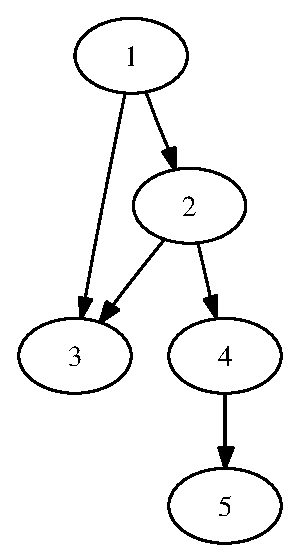
\epsfig{file=Figures/graph0,scale=0.5}
  \caption{A simple graph.}
  \label{fig:graph0}
\end{figure}

\noindent
The graph in figure \ref{fig:graph0} does only show the immediate connections between two
locations.  Of course, there are other connections which are, however, not immediate
connections.  For example, there is a path from location 
\texttt{1} to location \texttt{4} that visits the location \texttt{2}. 
We will represent this path as the list
\\[0.2cm]
\hspace*{1.3cm}
$[1,2,4]$.
\\[0.2cm]
In general, a path from $x$ to $z$ in the graph given by the relation $R$ is a list of the form
\\[0.2cm]
\hspace*{1.3cm}
$[ y_1, \cdots, y_n ]$
\\[0.2cm]
such that we have the following:
\begin{enumerate}
\item $y_1 = x$,
\item $y_n = z$, \quad and
\item $\forall i \in \{ 1, \cdots, n_1 \}: \pair(y_i, y_{i+1}) \el R$.
\end{enumerate}
Our goal is to develop a program that receives as input a binary relation $R$ representing a graph and
two locations $x$ and $y$.  The job of this program is to check whether there is a
connection from $x$ to $y$.  If a connection between $x$ and $y$ exists, the program
should also compute the corresponding path.


\subsection{Computing the Transitive Closure}
To begin with, we observe that there is a connection from location $x$ to location $y$ iff
\\[0.2cm]
\hspace*{1.3cm}
$\pair(x,y) \in R^+$,
\\[0.2cm]
where $R^+$ is the transitive closure of $R$.  In the last chapter, we have shown that the
transitive closure of $R$ can be defined as: \\[0.2cm]
\hspace*{1.3cm}
$R^+ = \bigcup\limits_{i=1}^{\infty} R^i = R \cup R^2 \cup R^3 \cup \cdots$
\\[0.2cm]
At first glance this looks as if the computation of $R^+$ requires an infinite
computation.  But let us try to dissect the infinite union of sets in the definition of $R^+$:
First, there is the set $R$.  These are all immediate connections.  Then we have $R^2$,
which is the same as $R \circ R$.  Now this is defined as \\[0.2cm]
\hspace*{1.3cm} $R \circ R = \{ \pair(x,z) \mid \exists y \colon \pair(x,y) \in R \wedge \pair(y,z) \in R \}$.
\\[0.2cm]
Therefore,  $R^2$ contains all those pairs $\pair(x,z)$ such that there is a path from
$x$ to $z$ with one stopover.  In general, we can show by induction on $n$ that
$R^n$ contains all those pairs $\pair(x,z)$ such that there are $n-1$ stopovers.
Now the set of locations is finite.  So there is some fixed number $k \in \mathbb{N}$
such that there are $k$ different locations.  But if there are only $k$ different
locations, when traveling from $x$ to $z$ there is no reason to consider more than $k-2$
stopovers, as otherwise we would visit a location twice.  Therefore, the formula for
computing $R^+$ can be shortened to
\\[0.2cm]
\hspace*{1.3cm} $R^+ = \bigcup\limits_{i=1}^{k-1} R^i$, 
\\[0.2cm]
provided there are only $k$ different locations.

We could use the formula given above.  However, it is more efficient to use a
\emph{fix-point algorithm}.  In order to do so, we verify that the transitive closure $R^+$
satisfies the following \emph{fix-point equation}:
\begin{equation}
  \label{fixpunkt}
  R^+ = R \cup R \circ R^+. 
\end{equation}
Let me remind you that we have agreed that the relational composition operator ``$\circ$'' has
a higher precedence than the union operator ``$\cup$''.  Therefore, the expression $R \cup
R \circ R^+$ has to  
be read as $R \cup (R \circ R^+)$.

The fix-point equation  \ref{fixpunkt} can be proven algebraically.  We have
\[
\begin{array}{cll}
    & R \cup R \circ R^+ \\[0.2cm]
  = & R \cup R \circ \bigcup\limits_{i=1}^{\infty} R^i \\[0.4cm]
  = & R \cup R \circ \bigl(R^1 \cup R^2 \cup R^3 \cup \cdots \bigr) \\[0.2cm]
  = & R \cup \bigl(R \circ R^1 \cup R \circ R^2 \cup R \circ R^3 \cup \cdots \bigr) &
      \mbox{law of distributivity} \\[0.2cm]
  = & R \cup \bigl(R^2 \cup R^3 \cup  R^4 \cup \cdots \bigr) & \mbox{definition of $R^n$} \\[0.2cm]
  = & \bigcup\limits_{i=1}^{\infty} R^i \\[0.4cm]
  = & R^+
\end{array}
\]
We will use the equation \ref{fixpunkt} in order to compute the transitive closure $R^+$
iteratively.  In order to do so we define a sequence  $(T_n)_{n \in \mathbb{N}}$ by
induction on $n$:
\begin{enumerate}
\item[I.A.] $n = 1$: \hspace*{2.3cm} $T_1 := R$
\item[I.S.] $n \mapsto n+1$: \hspace*{1.6cm} $T_{n+1} := R \cup R \circ T_n$. 
\end{enumerate}
The relations $T_n$ can be written in terms of the relation $R$:
\begin{enumerate}
\item $T_1 = R$.
\item $T_2 = R \cup R \circ T_1 = R \cup R \circ R = R^1 \cup R^2$.
\item $\begin{array}[t]{lcl}
       T_3  & = & R \cup R \circ T_2 \\
            & = & R \cup R \circ (R^1 \cup R^2) \\
            & = & R^1 \cup R^2 \cup R^3. \\
       \end{array}
      $
\end{enumerate}
In general, we can prove by induction that 
\[ T_n = \bigcup\limits_{i=1}^{n} R^i \]
holds.  
The base case is immediate from the definition of  $T_1$.  The induction step works as follows:
\[ \begin{array}{lcll}
   T_{n+1} & = & R \cup R \circ T_n & \mbox{from the definition of $T_{n+1}$} \\[0.2cm]
           & = & R \cup R \circ \left(\bigcup\limits_{i=1}^{n} R^i\right) &
                 \mbox{by induction hypotheses} \\[0.4cm]
           & = & R \cup R^2 \cup \cdots \cup R^{n+1}  &
                 \mbox{law of distributivity} \\[0.2cm]
           & = & \bigcup\limits_{i=1}^{n+1} R^i & \Box 
   \end{array}
\]
The sequence  $(T_n)_{n\in\mathbb{N}}$ is \emph{monotonically increasing}.  In general, a
sequence of sets $(X_n)_{n\in\mathbb{N}}$ is called \emph{monotonically increasing} iff we
have
\\[0.2cm]
\hspace*{1.3cm}
$\forall n \in \mathbb{N}: X_n \subseteq X_{n+1}$.
\\[0.2cm]
The fact that the sequence $(T_n)_{n\in\mathbb{N}}$ is monotonically increasing is an
immediate consequence of
\\[0.2cm]
\hspace*{1.3cm}
$T_n = \bigcup_{i=1}^{n} R^i$
\\[0.2cm]
as we have the following:
\\[0.2cm]
\hspace*{1.3cm}
$
\begin{array}[t]{llcl}
                & T_n \subseteq T_{n+1} \\[0.2cm]
\Leftrightarrow & \bigcup\limits_{i=1}^{n} R^i \subseteq \bigcup_{i=1}^{n+1} R^i \\[0.5cm]
\Leftrightarrow & \bigcup\limits_{i=1}^{n} R^i \subseteq \bigcup_{i=1}^{n} R^i \cup R^{n+1}. \\
\end{array}
$
\\[0.2cm]
If the relation $R$ is finite, of course  $R^+$ is finite, too.  All sets  $T_n$ are 
subsets of $T^+$, because we have 
\\[0.2cm]
\hspace*{1.3cm}
$T_n = \bigcup\limits_{i=1}^{n} R^i \subseteq \bigcup\limits_{i=1}^{\infty} R^i = R^+$ \quad for all $n \in \mathbb{N}$.
\\[0.2cm]
Therefore, the relations  $T_n$ can not get arbitrarily big.  As the sequence 
$(T_n)_{n\in\mathbb{N}}$ is monotonically increasing, there must be an index $k \in \mathbb{N}$ such that
all relations  $T_n$ are the same when $n \geq k$:
\\[0.2cm]
\hspace*{1.3cm}
$\forall n \in \mathbb{N}:( n \geq k \rightarrow T_n = T_k)$.
\\[0.2cm]
As we have $T_n = \bigcup_{i=1}^{n} R^i$, we conclude that
\\[0.2cm]
\hspace*{1.3cm}
$T_n = \bigcup\limits_{i=1}^{n} R^i = \bigcup\limits_{i=1}^{k} R^i = T_k$ \quad for all $n \geq k$.
\\[0.2cm]
This implies
\\[0.2cm]
\hspace*{1.3cm}
$T_n = \bigcup\limits_{i=1}^{n} R^i = \bigcup\limits_{i=1}^{\infty} R^i = R^+$. 
\quad for all $n \geq k$  
\\[0.2cm]
The algorithm for computing the sequence $(T_n)_{n \in \mathbb{N}}$ is now as follows:  
We start with $T_1 := R$ and then compute $T_{n+1}$ using
\[ T_{n+1} := R \cup R \circ T_n. \]
This iteration is done until we have $T_{n+1} = T_n$, since then $T_n = R^+$.


\begin{figure}[!ht]
  \centering
\begin{Verbatim}[ codes         = {\catcode`$=3\catcode`_=8\catcode`^=7},
                  frame         = lines, 
                  framesep      = 0.3cm, 
                  labelposition = bottomline,
                  numbers       = left,
                  numbersep     = -0.2cm,
                  commandchars  = \\\{\},
                  xleftmargin   = 0.8cm,
                  xrightmargin  = 0.8cm,
                ]
    program main;
    
        R := \{ [1,2], [2,3], [1,3], [2,4], [4,5] \};
        print( "R = ", R );
        print( "computing transitive closure of R" );
        T := closure(R);
        print( "R+ = ", T );
    
        -- \emph{The procedure call} \texttt{closure}($R$) \emph{computes the transitive closure}
        -- \emph{of the binary relation} $R$.
        procedure closure(R);
            T := R;
            loop
                Old\_T := T;
                T     := R + product(R, T);
                if T = Old\_T then
                    return T;
                end if;
            end loop;
        end closure;

        -- \emph{The procedure call} \texttt{product($R1$, $R2$)} \emph{computes the relational}
        -- \emph{product $R1 \circ R2$.}
        procedure product(R1, R2);
            return \{ [x,z] : [x,y1] in R1, [y2,z] in R2 | y1 = y2 \};
        end product;
    
    end main;
\end{Verbatim} 
\vspace*{-0.3cm}
\caption{Computing the transitive closure.}  \label{fig:transitive.stl}
\end{figure} %\$

\noindent
The program \texttt{transitive.stl} in figure
\ref{fig:transitive.stl} on page \pageref{fig:transitive.stl} shows an implementation of the
algorithm described above.
When executing this program, we get the following result:
\begin{verbatim}
    R = {[2, 3], [4, 5], [1, 3], [2, 4], [1, 2]}
    R+ = {[1, 5], [2, 3], [4, 5], [1, 4], [1, 3], [2, 4], [1, 2], [2, 5]}
\end{verbatim}
The transitive closure  $R^+$ of the relation $R$ can now be interpreted as followed:  
The pair  $\pair(x,y)$ is a member of $R^+$ if there is a \emph{path} starting from 
$x$ leading to $y$.  
The  procedure $\textsl{product}()$ shows the most general form of a set definition using iterators.
In general, we can define a set as follows:
\\[0.2cm]
\hspace*{1.3cm}
$\{\; \textsl{expr} \;\texttt{:}\; [x^{(1)}_1, \cdots, x^{(1)}_{n(1)}] \;\texttt{in}\; s_1,
     \cdots, [x^{(k)}_1, \cdots, x^{(k)}_{n(k)}] \;\texttt{in}\; s_k \;\texttt{|}\;
     \textsl{cond} \;\}
$
\\[0.2cm]
Here, for all $i=1, \cdots, k$ the expression $s_i$ has to be a set of lists such that each of
those lists has the length $n(i)$.  When this expression is evaluated, the variables 
$x^{(i)}_1, \cdots, x^{(i)}_{n(i)}$ are bound to the values of the corresponding components in the
lists that are members of the sets $s_i$.  For example, the evaluation of
\begin{verbatim}
 s1 := { [ 1, 2, 3 ], [ 5, 6, 7 ] };
 s2 := { [ "a", "b" ], [ "c", "d" ] };
 M := { [ x1, x2, x3, y1, y2 ] : [ x1, x2, x3 ] in s1, [ y1, y2 ] in s2 | true };
\end{verbatim}
yields the following result for the set  \texttt{M} 
\begin{verbatim}
    { [1, 2, 3, "a", "b"], [5, 6, 7, "c", "d"],  
      [1, 2, 3, "c", "d"], [5, 6, 7, "a", "b"] }.
\end{verbatim}

If we use this general form to define a list we have to obey an important restriction:
All the variables occuring in the various lists $x^{(i)}_1, \cdots, x^{(i)}_{n(i)}$
have to be distinct, that is, all variables  $x^{(i)}_j$ have to be different from each other.
Therefore, the procedure \textsl{product} given above can not be implemented as follows:
\begin{Verbatim}[ frame         = lines, 
                  framesep      = 0.3cm, 
                  labelposition = bottomline,
                  numbers       = left,
                  numbersep     = -0.2cm,
                  commandchars  = \\\{\},
                  xleftmargin   = 0.8cm,
                  xrightmargin  = 0.8cm,
                ]
        procedure product(R1, R2);
            return \{ [x,z] : [x,y] in R1, [y,z] in R2 \};
        end product;
\end{Verbatim} 
The reason is that the variable \texttt{y} occurs twice here.  
We have solved this problem by using two distinct variables
 \texttt{y1} and \texttt{y2}.  In order to enforce that the values of these variables are the same
 we had to add the condition \texttt{y1 = y2}.


\subsection{Computing the Paths}
The program shown in figure \ref{fig:transitive.stl} computes the transitive closure and therefore
answers the question, whether there is a connection between two given locations.  However, in practice
we do not only want to know whether there is a connection between two locations $x$ and $y$, we also want to
compute the path leading from $x$ to $y$.    In order to
have a convenient description of the algorithm for computing a path, we define the following functions:
\begin{enumerate}
\item The function $\textsl{first}(p)$ computes the first element of the list $p$: \\[0.2cm]
      \hspace*{1.3cm} $\textsl{first}\bigl([x_1,\cdots,x_m]\bigr) = x_1$.
\item The function $\textsl{last}(p)$ computes the last element of the list $p$: \\[0.2cm]
      \hspace*{1.3cm} $\textsl{last}\bigl([x_1,\cdots,x_m]\bigl) = x_m$.
\item If  $p = [ x_1, \cdots, x_m ]$ and $q =[ y_1, \cdots, y_n ]$   are two paths such that
      $\textsl{first}(q) = \textsl{last}(p)$, we define the
      \emph{sum} of $p$ and $q$ as \\[0.2cm]
      \hspace*{1.3cm} $p \oplus q := [x_1, \cdots, x_m, y_2, \cdots, y_n ]$.
\end{enumerate}
If  $P_1$ and $P_2$ are sets of paths, we define the  \emph{path product} of
$P_1$ and $P_2$ as follows: 
\\[0.2cm]
\hspace*{1.3cm} 
$P_1 \bullet P_2 := \bigl\{\; p_1 \oplus p_2 \mid p_1 \in P_1 \wedge p_2 \in P_2 \wedge \textsl{last}(p_1) = \textsl{first}(p_2) \;\bigr\}$.
\\[0.2cm]
Note that the path product generalizes the notion of relational composition:
If $P_1$ and $P_2$ are relations, i.~e.~if they contain only lists of length two, then
$P_1 \bullet P_2 = P_1 \circ P_2$.


\begin{figure}[!ht]
  \centering
\begin{Verbatim}[ codes         = {\catcode`$=3\catcode`_=8\catcode`^=7},
                  frame         = lines, 
                  framesep      = 0.3cm, 
                  labelposition = bottomline,
                  numbers       = left,
                  numbersep     = -0.2cm,
                  commandchars  = \\\{\},
                  xleftmargin   = 0.8cm,
                  xrightmargin  = 0.8cm,
                ]
    program main;
        R := \{ [1,2], [2,3], [1,3], [2,4], [4,5] \};
        print( "R = ", R );
        print( "computing all paths" );
        P := closure(R);
        print( "P = ", P );
        
        procedure closure(R);
            P := R;
            loop
                Old\_P := P;
                P     := P + path\_product(R, P);
                if P = Old\_P then
                    return P;
                end if;
            end loop;
        end closure;
    
        procedure path\_product(P, Q);
            return \{ add(p, q) : p in P, q in Q | p(#p) = q(1) \};
        end path\_product;    
    
        procedure add(p, q);
            return p + q(2..);
        end add;
    
    end main;
\end{Verbatim} 
\vspace*{-0.3cm}
\caption{Computing all connections.}  \label{fig:path.stl}
\end{figure} %\$

\begin{figure}[!ht]
  \centering
  \epsfig{file=Figures/graph-zykl,scale=0.5}
  \caption{A cyclic graph.}
  \label{fig:graph-zykl}
\end{figure}

Now we can change the program from figure 
\ref{fig:transitive.stl} in a way that all possible paths between two locations are computed.
The resulting program \texttt{path.stl} is shown in figure \ref{fig:path.stl}.
Unfortunately,  this program does not work if the graph admits cycles.
Figure \ref{fig:graph-zykl} shows a graph containing a cycle.  In this graph,
there is an infinite number of paths starting at location  1 and leading to location 2: \\[0.2cm]
\hspace*{1.3cm} 
$[ 1, 2 ]$, $[ 1, 2, 4, 1, 2 ]$, 
$[ 1, 2, 4, 1, 2, 4, 1, 2 ]$, 
$[ 1, 2, 4, 1, 2, 4, 1, 2, 4, 1, 4 ]$, $\cdots$
\\[0.2cm]
Obviously, we can forget those paths that are cyclic and therefore contain one location multiple times.
In order to keep our sets finite, we have to eliminate these paths.


\begin{figure}[!ht]
  \centering
\begin{Verbatim}[ numbers       = none,
                  frame         = lines, 
                  framesep      = 0.3cm, 
                  labelposition = bottomline,
                  xleftmargin   = 0.0cm,
                  xrightmargin  = 0.0cm,
                ]
 procedure path_product(P, Q);
    return { add(p,q) : p in P, q in Q | p(#p) = q(1) and not cyclic(add(p,q)) };
 end path_product;    

 procedure cyclic(p);
    return #{ x : x in p } < #p;
 end cyclic;
\end{Verbatim} 
\vspace*{-0.3cm}
\caption{Computing all connections in s cyclic graph.}  
\label{fig:path-cyclic.stl}
\end{figure} %\$

Figure \ref{fig:path-cyclic.stl} shows how the program has to be changed to make it work even for
graphs containing cycles. 
\begin{enumerate}
\item In line 2, we just collect those paths that are not cyclic.
\item In line 6 we check, whether a path is cyclic.  Now a path is cyclic iff it contains a
      location multiple times.  Therefore, if we transform a cyclic path into a set, the set
      will contain less elements than the path we started with.  The reason is that a set contains
      every element exactly once.
\end{enumerate}
In general, we are not interested to compute all connections between every possible pair of
locations $x$ and $y$.  Instead, we often have a starting location $x$ and a goal location $y$ and
we want to compute a path leading from $x$ to $y$.
The program \texttt{find-path.stl} shown in figure \ref{fig:find-path.stl} shows the implementation
of the procedure  $\texttt{reachable}(x, y, R)$.  This procedure checks whether there is a
path from $x$ to $y$ in the graph $R$.  Furthermore, a path is computed, provided there is
one. 
\begin{enumerate}
\item Line 3 initializes $P$ to contain the path of length 0 that starts and end with $x$.
\item Line 7 selects those paths from  $P$ that reach the location $y$.
\item If the set of those paths is not empty, then we are done.
      Therefore, in this case, we just pick an arbitrary path leading to $y$ and return it.
\item If we cannot find any more paths, then we leave the procedure in line 12 with a \texttt{return}
      statement.  As we do not return any expression, the return value is $\Omega$ in this case.
\end{enumerate}

\begin{figure}[!ht]
  \centering
\begin{Verbatim}[ codes         = {\catcode`$=3\catcode`_=8\catcode`^=7},
                  frame         = lines, 
                  framesep      = 0.3cm, 
                  labelposition = bottomline,
                  numbers       = left,
                  numbersep     = -0.2cm,
                  commandchars  = \\\{\},
                  xleftmargin   = 0.8cm,
                  xrightmargin  = 0.8cm,
                ]
        -- \emph{Check whether there is a path from $x$ to $y$ in $R$ and compute it}.
        procedure reachable(x, y, R);
            P := \{ [x] \};
            loop
                Old\_P := P;
                P     := P + path\_product(P, R);
                Found := \{ p in P | p(#p) = y \};
                if Found /= \{\} then
                    return arb Found;
                end if;
                if P = Old\_P then
                    return;
                end if;
            end loop;
        end reachable;
\end{Verbatim} 
\vspace*{-0.3cm}
\caption{Computing the connections between two points.}  
\label{fig:find-path.stl}
\end{figure} %\$



%%% Local Variables: 
%%% mode: latex
%%% TeX-master: "logic"
%%% End: 

